\documentclass{beamer}

\usepackage{amsmath}
\usepackage{amssymb} 
\usepackage{graphicx}
\usepackage{hyperref} % Added for links
\hypersetup{
    colorlinks=true,
    linkcolor=blue,
    urlcolor=cyan,
}

% --- Define Title Elements HERE ---
\title{Proposal for a Multi-Arm Biomarker RCT}
\subtitle{Executive Summary Slides}
\author{}
\date{\today}

% Choose a theme (optional, default is fine)
%\usetheme{default} 

\begin{document}

% --- Slide 1: Title ---
\begin{frame}
  \titlepage % Display the title page using info defined above
\end{frame}

% --- Slide 2: Motivation --- % (Added pauses)
\begin{frame}{Motivation}
  \begin{itemize}
    \item \textbf{Goal:} Design a multi-arm RCT to validate treatment-predictive biomarkers in psychiatry. \pause
    \item \textbf{(1) Efficiency:} Validating known biomarker candidates is often more statistically efficient than discovering them \emph{de novo}. \pause
    \item \textbf{(2) Future Data:} Yields a rich dataset suitable for \emph{post-hoc} development of complex predictive models (which treatment for whom?).
  \end{itemize}
\end{frame}

% --- Slide 3: Model Setup --- % (Rewritten & Added pauses)
\begin{frame}{Model: Setup}
  \begin{itemize}
    \item \textbf{Trial Structure:} $J$ distinct experimental treatment arms and $K$ potentially relevant biomarkers. \pause
    \item \textbf{Key Principle:} Modeler \textbf{pre-specifies interaction pairs} $ (j, k) $ of interest, forming a set $\mathcal{I}$. \pause
    \item \textbf{Focus:} Encourages powering for specific, plausible interactions. \pause
    \item (See Executive Summary for details on assumptions.)
  \end{itemize}
\end{frame}

% --- Slide 4: Linear Model --- % (Rewritten & Added pauses)
\begin{frame}{Model: Linear Formulation}
  
  Trial powered based on this model (simplified form): 
  \pause
  \vspace{1em} % Added vertical space
  $$ % Use $$ for display math
  Y_i = \beta_0 + \sum_{j=1}^J \beta^{txt}_j T_{ij} + \sum_{k=1}^K \beta^{bio}_k X_{ik} + \sum_{(j,k) \in \mathcal{I}} \beta^{int}_{jk} T_{ij} X_{ik} + \varepsilon_i 
  $$ % Use $$ for display math
  \pause
  \vspace{1em} % Added vertical space
  \textbf{Key Term:} $ \beta^{int}_{jk} $ represents the interaction effect for pre-specified pairs $ (j,k) \in \mathcal{I} $. % Use $ for inline math
  \pause
  \vfill % Add vertical space if needed
  (See Executive Summary for full coefficient interpretation.)
  
\end{frame}

% --- Slide 5: Coefficient Interpretation --- % (New Frame, Added pauses)
\begin{frame}{Model: Coefficient Interpretation}
  Based on the model:
  $$ Y_i = \beta_0 + \sum_{j=1}^J \beta^{txt}_j T_{ij} + \sum_{k=1}^K \beta^{bio}_k X_{ik} + \sum_{(j,k) \in \mathcal{I}} \beta^{int}_{jk} T_{ij} X_{ik} + \varepsilon_i $$
  \vspace{1em}
  \begin{itemize}
      \item $\beta_0$ : Average outcome for the reference treatment group. \pause
      \item $\beta^{txt}_j$: Main effect of treatment $j$ vs. reference. \pause
      \item $\beta^{bio}_k$: General association of biomarker $k$ with outcome (prognostic effect; control). \pause
      \item $\mathbf{\beta^{int}_{jk}}$: \textbf{Interaction effect} (Primary Target!) - How biomarker $k$ modulates treatment $j$'s effect, for pre-specified $(j,k) \in \mathcal{I}$.
  \end{itemize}
\end{frame}


% --- Slide 6: Interactive App --- % (Added pauses)
\begin{frame}{Interactive Power Simulation App}
  \begin{itemize}
      \item To explore design choices, especially \textbf{unequal sample sizes} per arm, an interactive Shiny app was developed. \pause
      \item Allows specifying J, K, interaction strengths (grid), individual arm sizes ($n_j$), and simulation parameters. \pause
      \item Reports power per interaction and overall power (ANY/ALL) via Holm. \pause
      \item App available via link in Executive Summary. % Plain text reference
  \end{itemize}
  \vfill % Push figure towards bottom if space allows
  \begin{figure}
      \centering
      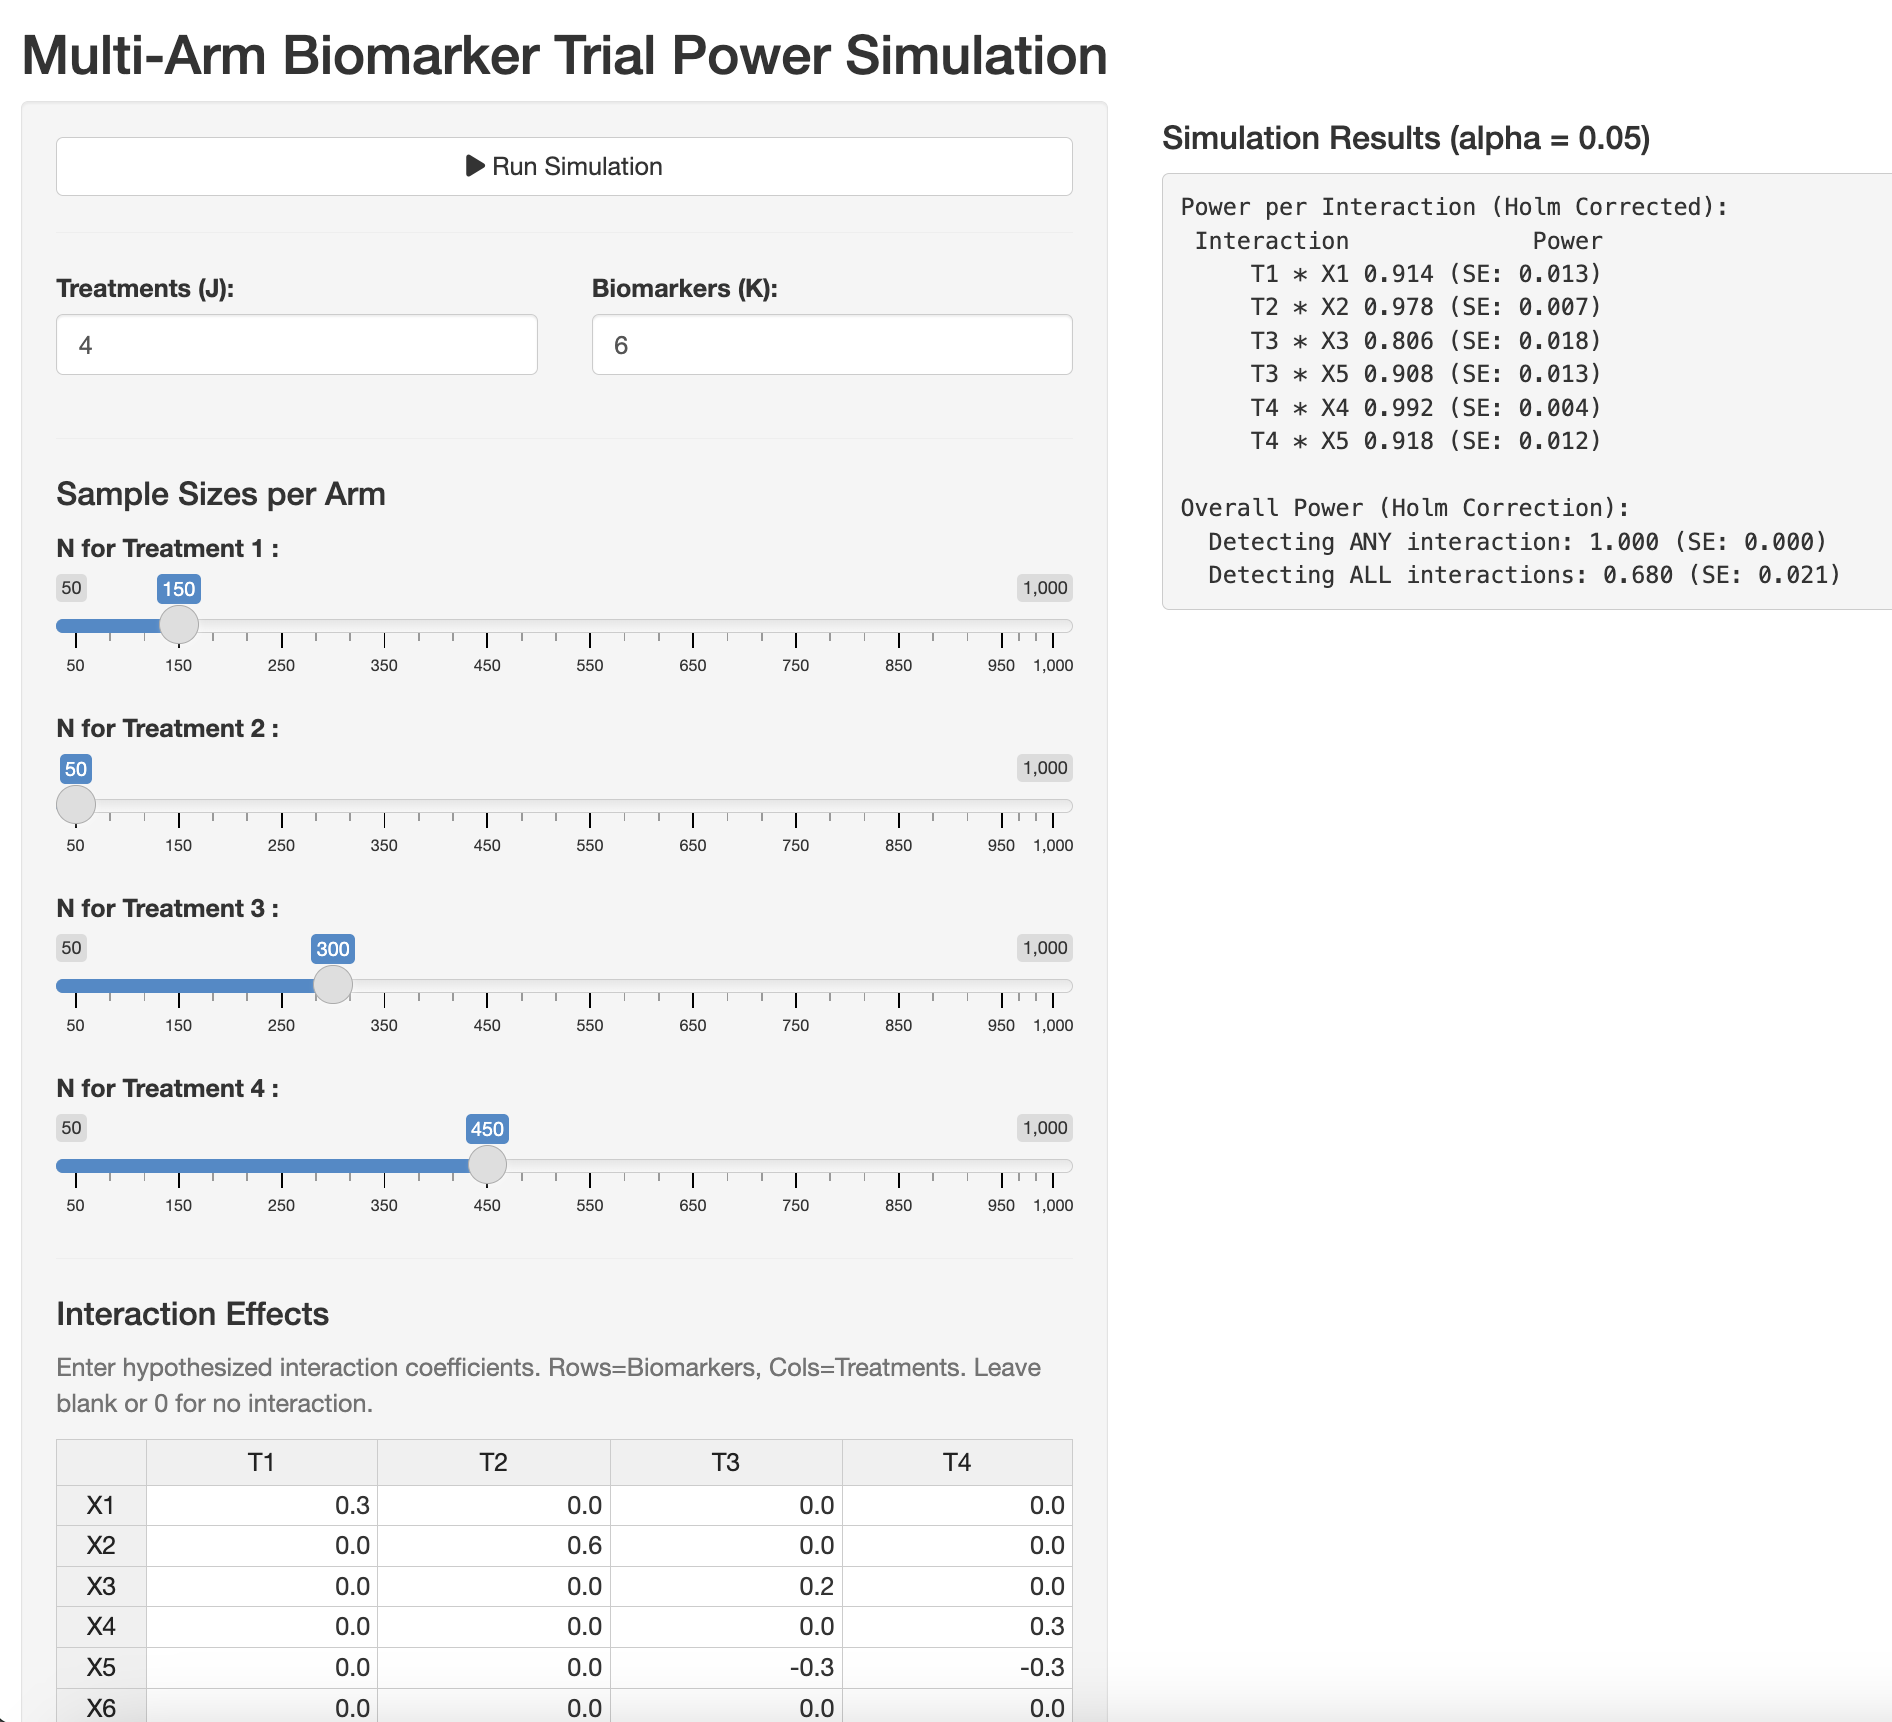
\includegraphics[width=0.8\textwidth]{figs/app.png}
      \caption{App showing J=4, K=5 scenario with unequal N. Power(ALL) $\approx$ 0.6.}
  \end{figure} 
\end{frame}

% --- Slide 7: Conclusion --- % (Added pauses)
\begin{frame}{Summary \& Next Steps} % Escaped ampersand
    \begin{itemize}
        \item Designing trials around pre-specified interactions $\mathcal{I}$ allows focused power calculations. \pause
        \item Unequal sample sizes can be explored via the simulation app to potentially improve efficiency. \pause
        \item Key decisions involve selecting interactions $\mathcal{I}$ and the overall success criterion (ANY vs. ALL). \pause
        \item \textbf{Please see the Executive Summary document for detailed rationale, model interpretation, and further discussion.}
    \end{itemize}
\end{frame}

\end{document} 